%%%%%%%%%%%%%%%%%%%%%%%%%%%%%%%%%%%%%%%%%
% Beamer Presentation
% LaTeX Template
% Version 1.0 (10/11/12)
%
% This template has been downloaded from:
% http://www.LaTeXTemplates.com
%
% License:
% CC BY-NC-SA 3.0 (http://creativecommons.org/licenses/by-nc-sa/3.0/)
%
%%%%%%%%%%%%%%%%%%%%%%%%%%%%%%%%%%%%%%%%%

\documentclass[t]{beamer}

\usepackage[english]{babel}
\usepackage[utf8]{inputenc}
\usepackage{hyperref}
\usepackage{verbatim}
\usepackage{listings}

%----------------------------------------------------------------------------------------
%	PACKAGES AND THEMES
%----------------------------------------------------------------------------------------

\mode<presentation> {

% The Beamer class comes with a number of default slide themes
% which change the colors and layouts of slides. Below this is a list
% of all the themes, uncomment each in turn to see what they look like.

%\usetheme{default}
%\usetheme{AnnArbor}
%\usetheme{Antibes}
%\usetheme{Bergen}
%\usetheme{Berkeley}
%\usetheme{Berlin}
%\usetheme{Boadilla}
%\usetheme{CambridgeUS}
%\usetheme{Copenhagen}
%\usetheme{Darmstadt}
%\usetheme{Dresden}
%\usetheme{Frankfurt}
%\usetheme{Goettingen}
%\usetheme{Hannover}
%\usetheme{Ilmenau}
%\usetheme{JuanLesPins}
%\usetheme{Luebeck}
%\usetheme{Madrid}
%\usetheme{Malmoe}
%\usetheme{Marburg}
%\usetheme{Montpellier}
%\usetheme{PaloAlto}
%\usetheme{Pittsburgh}
%\usetheme{Rochester}
%\usetheme{Singapore}
%\usetheme{Szeged}
\usetheme{Warsaw}

% As well as themes, the Beamer class has a number of color themes
% for any slide theme. Uncomment each of these in turn to see how it
% changes the colors of your current slide theme.

%\usecolortheme{albatross}
%\usecolortheme{beaver}
%\usecolortheme{beetle}
%\usecolortheme{crane}
%\usecolortheme{dolphin}
%\usecolortheme{dove}
%\usecolortheme{fly}
%\usecolortheme{lily}
%\usecolortheme{orchid}
%\usecolortheme{rose}
\usecolortheme{seagull}
%\usecolortheme{seahorse}
%\usecolortheme{whale}
%\usecolortheme{wolverine}

\usefonttheme{structuresmallcapsserif}

%\setbeamertemplate{footline} % To remove the footer line in all slides uncomment this line
%\setbeamertemplate{footline}[page number] % To replace the footer line in all slides with a simple slide count uncomment this line

%\setbeamertemplate{navigation symbols}{} % To remove the navigation symbols from the bottom of all slides uncomment this line
}


\usepackage{graphicx} % Allows including images
\usepackage{booktabs} % Allows the use of \toprule, \midrule and \bottomrule in tables



\lstdefinestyle{cpp}{
  language=C++,
  basicstyle=\ttfamily\footnotesize,  % Use small true type font
  showstringspaces=false,                 % Don't put marks in string spaces
  tabsize=2,                              % 5 spaces per tab
  escapeinside={@}{@},                % for invisible labels
  breaklines=true,
  breakatwhitespace=true,
  emptylines=1,
  texcl=true,
  escapechar=@,
  mathescape=true,
  xleftmargin=2.5ex,
  keywordstyle=[1]\color{blue},
  % keywordstyle=[2]\color{red},
	% stringstyle=\color{red},
	% commentstyle=\color{green},
	% morekeywords=[1]{pop_front}
	% morekeywords=[2]{parent,child}
}

\usepackage{wrapfig}
\author[]{Kevin Wallimann \quad Johannes Baum \quad Matthias Untergassmair}

%----------------------------------------------------------------------------------------
%	TITLE PAGE
%----------------------------------------------------------------------------------------

\title[Topological Sorting]{Parallel Topological Sorting} % The short title appears at the bottom of every slide, the full title is only on the title page
\subtitle{Design of High Performance Computing, Fall 2015}

\institute[ETHZ]{ ETH Zürich }
%\date{\today} % Date, can be changed to a custom date
\date{December 14, 2015}
	\begin{document}

\begin{frame}
\titlepage % Print the title page as the first slide
\end{frame}

%----------------------------------------------------------------------------------------
%	PRESENTATION SLIDES
%----------------------------------------------------------------------------------------

%------------------------------------------------
\section{Overview}
%------------------------------------------------


\begin{frame}
\frametitle{Overview}

\begin{itemize}
\item DAG defines partial order
\item Topological sorting defines one total order on a DAG
\item Parallel algorithm: finds one topological sorting of a given DAG
\end{itemize}

\end{frame}

%------------------------------------------------
\section{Difference to BFS}
%------------------------------------------------

\begin{frame}
\frametitle{Difference to BFS}

\begin{itemize}
\item BFS visits every node
\item Topological sorting algorithm needs to visit every edge
\end{itemize}

Example:

\begin{figure}[!hbp]
 
  \begin{tikzpicture}[->,>=stealth',auto,node distance=1cm,
                    thick,main
                    node/.style={circle,draw,font=\sffamily\scriptsize},text node/.style={draw=none,font=\sffamily\tiny}]

  \node[main node] (1) [draw=black!80,text=black!80] {A};
  \node[main node] (2) [below right of=1, node distance=1.2cm]{B};
  \node[main node] (3) [below of=1, node distance=1.2cm] {C};
  

  \path[every node/.style={font=\sffamily\small}]
    (1) edge (2)
    (2) edge (3)
    (1) edge (3)
    ;
\end{tikzpicture}

\end{figure}

Consider order A,C,B
$\rightarrow$ valid in BFS, invalid in topological sorting


\end{frame}

%------------------------------------------------
\section{Input graphs}
%------------------------------------------------
%TODO: Maybe omit random graph at all
\begin{frame}
\frametitle{Random graph}
\begin{columns}[c]
 \column{0.29\textwidth}
 \begin{tabular}{p{1cm}p{1cm}p{1.5cm}}
  Nodes    & Edges   & Degree (Median)\\\hline
  100'000  & 266'699 & 2\\
  10'000   & 26'989 & 2
 \end{tabular}
 \column{0.7\textwidth}
 \begin{figure}[!hbp]
    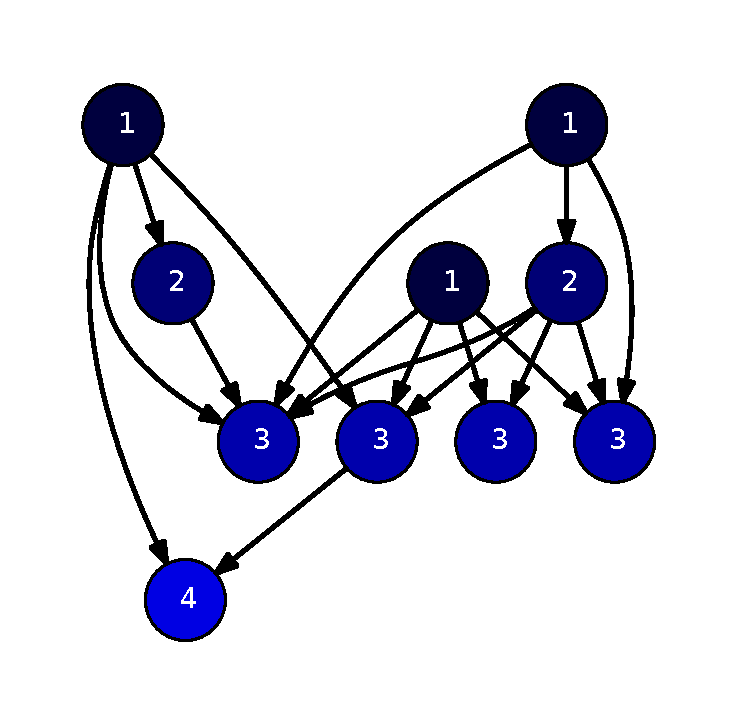
\includegraphics[height=0.7\textheight]{img/random_lin10.pdf}
 \end{figure}
\end{columns}

\end{frame}

\begin{frame}
\frametitle{Software dependency graph}
\begin{columns}[c]
 \column{0.29\textwidth}
 \begin{tabular}{p{1cm}p{1cm}p{1.5cm}}
  Nodes    & Edges   & Degree (Median)\\\hline
  100'000  & 266'680 & 2\\
  10'000   & 27'416  & 2
 \end{tabular}
 \column{0.7\textwidth}
 \begin{figure}[!hbp]
    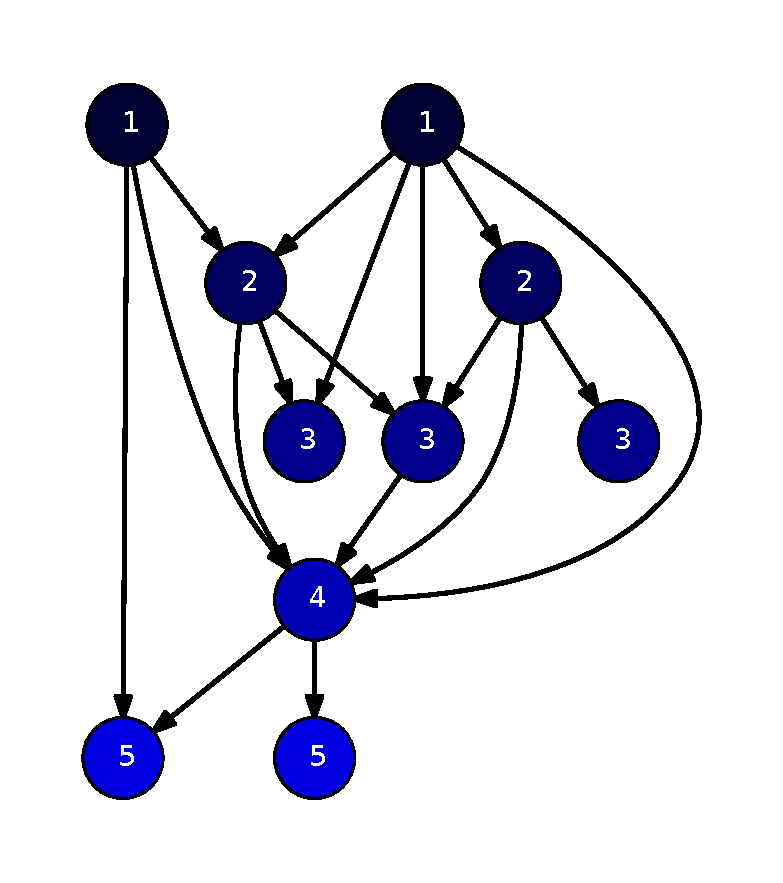
\includegraphics[height=0.7\textheight]{img/software10.pdf}
 \end{figure}

\end{columns}


{\color{gray}\tiny Musco, V. et al. (2014) "A Generative Model of Software Dependency Graphs to Better Understand Software Evolution."}
\end{frame}


%------------------------------------------------
\section{Implementations}
%------------------------------------------------

\begin{frame}
\frametitle{Parallel algorithm (shared memory)}
\begin{columns}[T]
 \column{0.5\textwidth}
  \begin{enumerate}
    \item As a preparing step, initialize a counter for every child with the number of its parents.
    \item Distribute parent nodes over threads and process them in parallel.
    \item For every parent, append it to solution.
    \item For every child of the parent, decrement its counter. If the counter is zero, make it a parent.
    \item Distribute new parent nodes etc.
  \end{enumerate}

 \column{0.5\textwidth}
  \begin{figure}[!ht]
    \begin{center}
      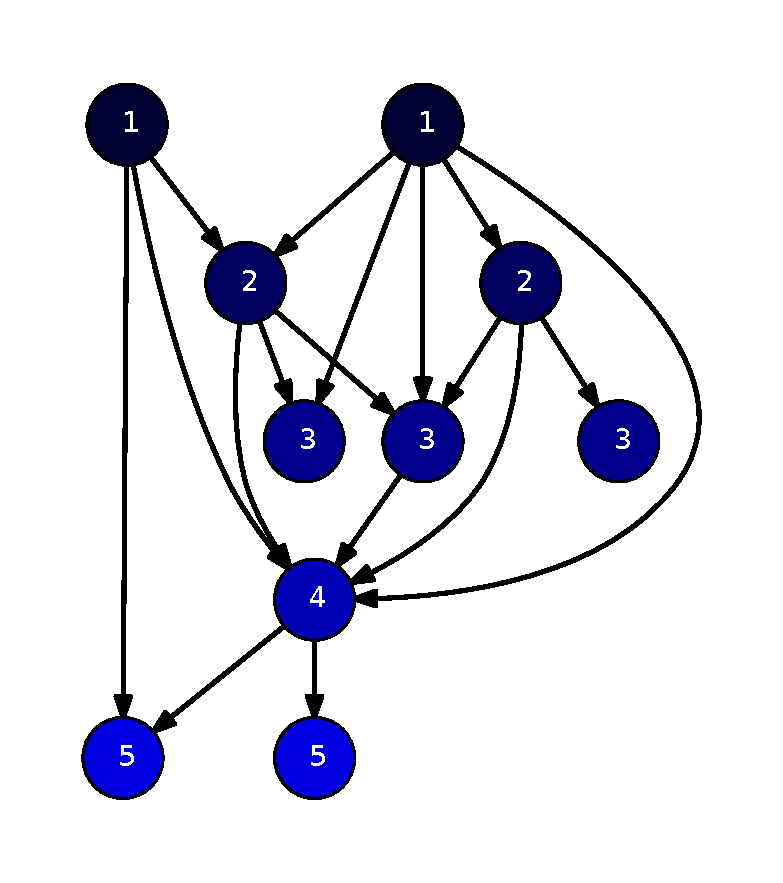
\includegraphics[width=0.9\textwidth]{img/software10.pdf}
    \end{center}
  \end{figure}
\end{columns}

\end{frame}


\begin{frame}
 \frametitle{Local lists approach}
  \begin{itemize}
  \item Parent nodes stored in a shared list.
  \item Distribution of parent nodes: Scatter the list among the threads. Each thread has now its local list.
  \item Add new parents to the end of local list.
  \item When all parents were processed, gather all local lists into the shared list.
  \item Repeat until there are no parents in the shared list.
  \end{itemize}
\end{frame}

\begin{frame}
 \frametitle{Boolean array approach}
 \begin{itemize}
  \item Array of length $N$. 1 if node $i$ is a parent node, 0 otherwise.
  \item Distribution of parent nodes: Parallel for-loop through the array.
  \item Mark new parents by setting a 1 in a second array.
  \item When all parents were processed, swap arrays.
  \item Loop through the array until there are no new parents.
 \end{itemize}
\end{frame}

\begin{frame}[fragile]
 \frametitle{Optimistic counter check}
 \begin{itemize}
  \item Decrement shared counter
  \item Return true if counter is zero
 \end{itemize}
 \begin{lstlisting}[style=cpp]
  inline bool counterCheck() {
          bool lastone;
          #pragma omp critical
          {
            --parcount_;
            lastone = (parcount_ == 0);
          }
          return lastone;
  }
 \end{lstlisting}
\end{frame}

\begin{frame}[fragile]
 \frametitle{Optimistic counter check}
 \begin{itemize}
  \item Decrement shared counter
  \item Return true if counter is zero
 \end{itemize}
 \begin{lstlisting}[style=cpp]
  inline bool counterCheck() {
          #pragma omp atomic
          --parcount_;
          return (parcount_ == 0);
  }
 \end{lstlisting}
 \begin{itemize}
  \item Multiple threads could return true, although only one thread should do so.
 \end{itemize}
\end{frame}

\begin{frame}[fragile]
 \frametitle{Optimistic counter check}
  \begin{lstlisting}[style=cpp]
  inline bool counterCheck() {
          #pragma omp atomic
          --parcount_;
          return (parcount_ == 0);
  }
 \end{lstlisting}
 \begin{itemize}
  \item List based approach: Child is inserted multiple times to solution $\Rightarrow$ Wrong.
  \item Array approach: Multiple threads write 1 to the array $\Rightarrow$ Ok, doesn't matter.
 \end{itemize}
\end{frame}

%------------------------------------------------
\section{Architecture}
%------------------------------------------------
\frametitle{Euler}
\begin{itemize}
 \item Intel Xeon E5 on Euler cluster
 \item 2 processors per node
 \item 12 cores
 \item 30 MB shared last-level cache
\end{itemize}


%------------------------------------------------
\section{Results}
%------------------------------------------------

\begin{frame}
\frametitle{Results - Xeon Phi}



\end{frame}


\end{document} 
